\documentclass[journal,12pt,twocolumn]{IEEEtran}
\usepackage{setspace}
\usepackage{gensymb}
\usepackage{xcolor}
\usepackage{caption}
\singlespacing
\usepackage{siunitx}
\usepackage[cmex10]{amsmath}
\usepackage{mathtools}
\usepackage{hyperref}
\usepackage{amsthm}
\usepackage{mathrsfs}
\usepackage{txfonts}
\usepackage{stfloats}
\usepackage{cite}
\usepackage{cases}
\usepackage{subfig}
\usepackage{longtable}
\usepackage{multirow}
\usepackage{enumitem}
\usepackage{bm}
\usepackage{mathtools}
\usepackage{listings}
\usepackage{tikz}
\usetikzlibrary{shapes,arrows,positioning}
\usepackage{circuitikz}
\renewcommand{\vec}[1]{\boldsymbol{\mathbf{#1}}}
\DeclareMathOperator*{\Res}{Res}
\renewcommand\thesection{\arabic{section}}
\renewcommand\thesubsection{\thesection.\arabic{subsection}}
\renewcommand\thesubsubsection{\thesubsection.\arabic{subsubsection}}

\renewcommand\thesectiondis{\arabic{section}}
\renewcommand\thesubsectiondis{\thesectiondis.\arabic{subsection}}
\renewcommand\thesubsubsectiondis{\thesubsectiondis.\arabic{subsubsection}}
\hyphenation{op-tical net-works semi-conduc-tor}

\lstset{
language=Python,
frame=single, 
breaklines=true,
columns=fullflexible
}
\begin{document}
\theoremstyle{definition}
\newtheorem{theorem}{Theorem}[section]
\newtheorem{problem}{Problem}
\newtheorem{proposition}{Proposition}[section]
\newtheorem{lemma}{Lemma}[section]
\newtheorem{corollary}[theorem]{Corollary}
\newtheorem{example}{Example}[section]
\newtheorem{definition}{Definition}[section]
\newcommand{\BEQA}{\begin{eqnarray}}
        \newcommand{\EEQA}{\end{eqnarray}}
\newcommand{\define}{\stackrel{\triangle}{=}}
\newcommand{\myvec}[1]{\ensuremath{\begin{pmatrix}#1\end{pmatrix}}}
\newcommand{\mydet}[1]{\ensuremath{\begin{vmatrix}#1\end{vmatrix}}}
\bibliographystyle{IEEEtran}
\providecommand{\nCr}[2]{\,^{#1}C_{#2}} % nCr
\providecommand{\nPr}[2]{\,^{#1}P_{#2}} % nPr
\providecommand{\mbf}{\mathbf}
\providecommand{\pr}[1]{\ensuremath{\Pr\left(#1\right)}}
\providecommand{\qfunc}[1]{\ensuremath{Q\left(#1\right)}}
\providecommand{\sbrak}[1]{\ensuremath{{}\left[#1\right]}}
\providecommand{\lsbrak}[1]{\ensuremath{{}\left[#1\right.}}
\providecommand{\rsbrak}[1]{\ensuremath{{}\left.#1\right]}}
\providecommand{\brak}[1]{\ensuremath{\left(#1\right)}}
\providecommand{\lbrak}[1]{\ensuremath{\left(#1\right.}}
\providecommand{\rbrak}[1]{\ensuremath{\left.#1\right)}}
\providecommand{\cbrak}[1]{\ensuremath{\left\{#1\right\}}}
\providecommand{\lcbrak}[1]{\ensuremath{\left\{#1\right.}}
\providecommand{\rcbrak}[1]{\ensuremath{\left.#1\right\}}}
\theoremstyle{remark}
\newtheorem{rem}{Remark}
\newcommand{\sgn}{\mathop{\mathrm{sgn}}}
\newcommand{\rect}{\mathop{\mathrm{rect}}}
\newcommand{\sinc}{\mathop{\mathrm{sinc}}}
\providecommand{\abs}[1]{\left\vert#1\right\vert}
\providecommand{\res}[1]{\Res\displaylimits_{#1}}
\providecommand{\norm}[1]{\lVert#1\rVert}
\providecommand{\mtx}[1]{\mathbf{#1}}
\providecommand{\mean}[1]{E\left[ #1 \right]}
\providecommand{\fourier}{\overset{\mathcal{F}}{ \rightleftharpoons}}
\providecommand{\ztrans}{\overset{\mathcal{Z}}{ \rightleftharpoons}}
\providecommand{\system}[1]{\overset{\mathcal{#1}}{ \longleftrightarrow}}
\newcommand{\solution}{\noindent \textbf{Solution: }}
\providecommand{\dec}[2]{\ensuremath{\overset{#1}{\underset{#2}{\gtrless}}}}
\let\StandardTheFigure\thefigure
\def\putbox#1#2#3{\makebox[0in][l]{\makebox[#1][l]{}\raisebox{\baselineskip}[0in][0in]{\raisebox{#2}[0in][0in]{#3}}}}
\def\rightbox#1{\makebox[0in][r]{#1}}
\def\centbox#1{\makebox[0in]{#1}}
\def\topbox#1{\raisebox{-\baselineskip}[0in][0in]{#1}}
\def\midbox#1{\raisebox{-0.5\baselineskip}[0in][0in]{#1}}

\vspace{3cm}
\title{12.6.3.18}
\author{Lokesh Surana}
\maketitle
\section*{Class 12, Chapter 6, Exercise 3.18}

Q. A rectangular sheet of tin 45 cm by 24 cm is to be made into a box without top, by cutting off square from each corner and folding up the flaps. What should be the side of the square to be cut off so that the volume of the box is maximum ?

\solution The length of sheet is 45 cm $\brak{\text{Let } a}$ and breadth of sheet is 24 cm $\brak{\text{Let }b}$.

\begin{figure}[!htb]
    \centering
    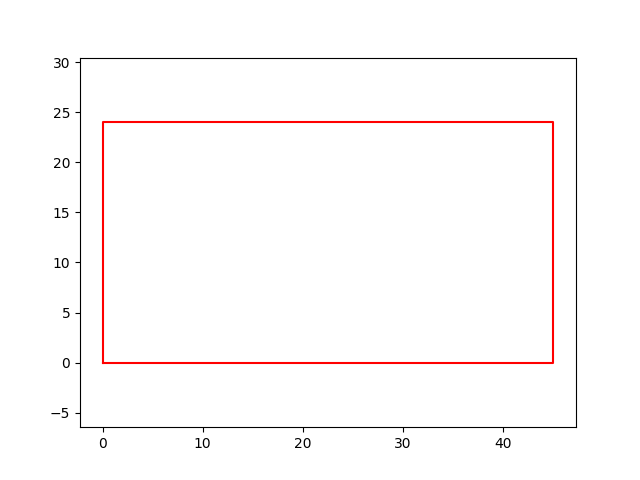
\includegraphics[width=\columnwidth]{figs/rectangle1.png}
    \caption{Rectangular sheet}
    \label{fig:rectangular sheet}
\end{figure}

Here is the figure of how the rectangular sheet will look if we cut equal sized square from each corner, ref \eqref{fig:rectangular sheet cut}

\begin{figure}[!htb]
    \centering
    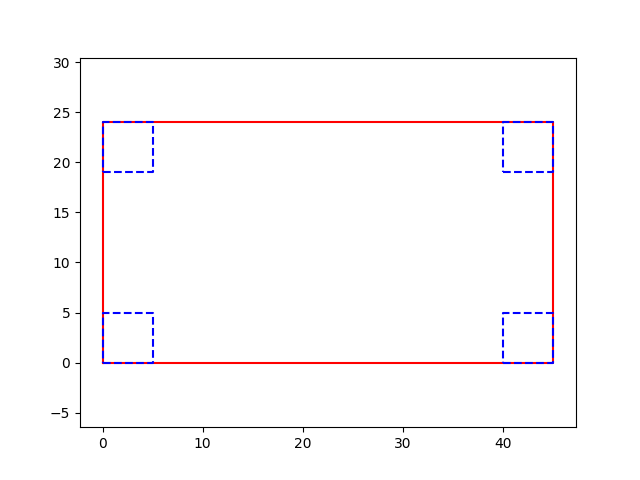
\includegraphics[width=\columnwidth]{figs/rectangle2.png}
    \caption{Rectangular sheet after cut}
    \label{fig:rectangular sheet cut}
\end{figure}

The new legnth, breadth and height of the box will be $a-2x$ $\brak{\text{Let }l}$, $b-2x$ $\brak{\text{Let }b}$ and $x$ $\brak{\text{Let }h}$ respectively.

\begin{align}
    \text{Volume of the box} &= l \times b \times h \\
    & = (a-2x) \times (b-2x) \times x \\
    \label{eq:volume} & = 4x^3 - 2\brak{a+b}x^2 + abx
\end{align}

From the figure , we can see that
\begin{align}
    \label{eq:x_range}
    0 < x \leq \min\brak{a,b}/2
\end{align}

Now, we have to find the side of the square to be cut off so that the volume of the box is maximum. So we have to find maxima of equation \eqref{eq:volume}.

Finding the maxima of equation \eqref{eq:volume} is same as finding the minima of equation \eqref{eq:volume} multiplied by $-1$, i.e. \eqref{eq:neg_volume}).

\begin{align}
    \label{eq:neg_volume}
    f\brak{x} &= -4x^3 + 2\brak{a+b}x^2 - abx
\end{align}

Using the given values of $a$ and $b$, we get
\begin{align}
    \label{eq:neg_volume2}
    f\brak{x} &= -4x^3 + 138x^2 - 1080x
\end{align}

The derivative of the function is
\begin{align}
    f^\prime\brak{x} &= -12x^2 + 276x - 1080 
\end{align}

Minima of \eqref{eq:neg_volume2} using gradient descent method is

\begin{align}
	\lambda_{n+1} &= \lambda_n - \alpha f^\prime\brak{\lambda_n}\\
    \label{eq:grad_dec/eq1}
    &= \lambda_n - \alpha \brak{-12\lambda_n^2 + 276\lambda_n - 1080}\\
\end{align}

Choosing
\begin{enumerate}
 \item $\alpha$ = 0.001
 \item precision = 0.0000001
 \item n = 10000000 
 \item $\lambda_0$ = 0
\end{enumerate}

\begin{align}
    \lambda_{min} &= 5
\end{align}

$x=5$ is the point of minima of the $f\brak{x}$.
So, it's point of maxima for the volume of the box.

\begin{figure}[!htb]
    \centering
    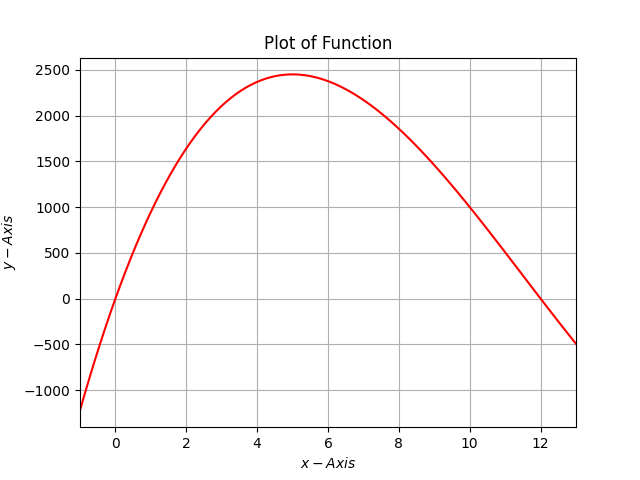
\includegraphics[width=\columnwidth]{figs/plot.png}
    \caption{Plot of volume function}
    \label{fig:plot of function}
\end{figure}

\end{document}